\documentclass[12pt]{article}
\usepackage[utf8]{inputenc}
%\usepackage[ngerman]{babel}
%\usepackage[utopia,sfscaled]{mathdesign}
%\usepackage[lf,minionint]{MinionPro}
%\renewcommand{\sfdefault}{phv}
%\usepackage[lf]{MyriadPro}
\usepackage{multicol, array}
\newcolumntype{C}{>{$}c<{$}} % math-mode version of "c" column type
\newcolumntype{L}{>{$}l<{$}} % math-mode version of "l" column type
%\usepackage[top=1cm,bottom=1in,left=1cm,right=1cm]{geometry}
\usepackage[margin=1in]{geometry} 

\usepackage{hyperref}
\usepackage{lipsum}
\usepackage[framemethod=tikz]{mdframed}
%\usepackage{fancyhdr} --$\rightarrow$ ???
\usepackage{microtype}
\usepackage{amsmath,amsthm,amssymb, mathrsfs} % for math

% \usepackage{dirtree} % for directory trees

\usepackage{graphicx} % Allows including images
% \graphicspath{ {image/} }
%\usepackage{booktabs} % Allows the use of \toprule, \midrule and \bottomrule in tables
\DeclareGraphicsExtensions{.pdf,.png,.jpg}


\newcommand{\N}{\mathbb{N}}
\newcommand{\C}{\mathbb{C}}

\newcommand{\B}{\mathbb{B}}

\newcommand{\Z}{\mathbb{Z}}
\newcommand{\Q}{\mathbb{Q}}

\newcommand{\R}{\mathbb{R}}
\newcommand{\Md}{(M,d(x,y))}

\newcommand{\F}{\mathbb{F}}
\newcommand{\E}{\mathbb{E}}
\newcommand{\e}{\varepsilon}


\theoremstyle{definition}
\newtheorem{definition}{Defn}
%\newtheorem{theorem}{Thm}[section]
\newtheorem{theorem}{Thm}
\newtheorem{corollary}{Cor}[theorem]
\newtheorem{lemma}{Lemma}
\newtheorem{prop}{Prop}
\newtheorem{example}{Example}

\newenvironment{solution}
  {\begin{proof}[Solution.]}
  {\end{proof}}
\newenvironment{Definition}[1]
  {\begin{definition}{\textbf{#1}: }}
  {\end{definition}}
\newenvironment{Function}[1]
  {\begin{function}{\texttt{#1}: }}
  {\end{function}}

\usepackage[ruled,vlined,linesnumbered]{algorithm2e}
\SetKw{Continue}{continue}
\SetKw{DownTo}{downto}
\include{pythonlisting}

\DeclareMathOperator*{\argmax}{arg\,max}
\DeclareMathOperator*{\argmin}{arg\,min}

% Script r from Griffiths
\def\rcurs{{\mbox{$\resizebox{.09in}{.08in}{\includegraphics[trim= 1em 0 14em 0,clip]{ScriptR}}$}}}
\def\brcurs{{\mbox{$\resizebox{.09in}{.08in}{\includegraphics[trim= 1em 0 14em 0,clip]{BoldR}}$}}}
\def\hrcurs{{\mbox{$\hat \brcurs$}}}

% define different joins
\def\ojoin{\setbox0=\hbox{$\Join$}%
  \rule[-.02ex]{.25em}{.4pt}\llap{\rule[1.10ex]{.25em}{.4pt}}}
\def\leftouterjoin{\mathbin{\ojoin\mkern-8.5mu\Join}}
\def\rightouterjoin{\mathbin{\Join\mkern-8.5mu\ojoin}}
\def\fullouterjoin{\mathbin{\ojoin\mkern-8.5mu\Join\mkern-8.5mu\ojoin}}

\renewcommand{\baselinestretch}{1}
%\pagestyle{empty}


% \newcommand{\header}{
% \begin{mdframed}[style=header]
% \footnotesize
% Some Text Inside\\
% Page~\thepage~of~6
% \end{mdframed}
% }


\newenvironment{problem}[2][Problem]{\begin{trivlist}
\item[\hskip \labelsep {\bfseries #1}\hskip \labelsep {\bfseries #2.}]}{\end{trivlist}}
\usepackage{setspace}



\begin{document}
 
\title{AHRQ Vinci guide}
\author{Max Yu}
\date{}
\maketitle

This document is a compilation of various VINCI related guides. Most of the following info is available on Slack under the ``vinci-technical'' channel, pulled from guides from Andy, Justin, and Paarth. 

% \setcounter{tocdepth}{1} % display subsubsections as well
\tableofcontents
% \setcounter{section}{-1}




\section{Log On and Setup}
\subsection{Citrix General Desktop}
In order to log on through personal equipment, one needs:
\begin{itemize}
    \item CAG access
    \item A PIV card reader. e.g. \url{https://www.amazon.com/gp/product/B002N3MM6W/ref=ppx_yo_dt_b_search_asin_title?ie=UTF8&psc=1}
    \item PIV badge + other accesses
    \item Download citrix workspace app. \url{https://raportal.vpn.va.gov/}
\end{itemize} 

Then go to \url{https://citrixaccess.va.gov/vpn/index_citrix_splash.html} to log on, selecting `click here to use Smartcard'.

After logging in, select the `1VA-General Desktop' 

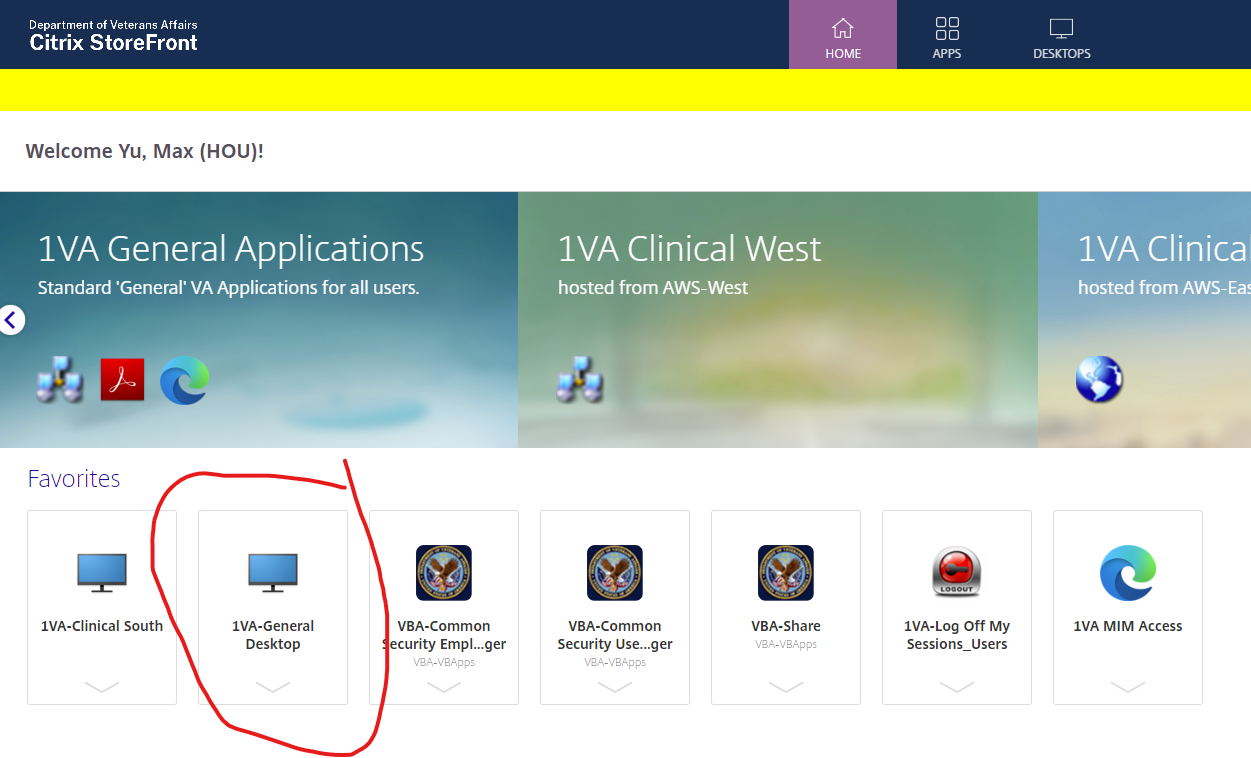
\includegraphics[width=\linewidth]{screenshots/citrix-logon-general-desktop.png}


On Mac there will be a downloaded ica file. Click to open. (Windows should automatically open. )

The Citrix Desktop has a few uses:
\begin{itemize}
    \item Proxy for VINCI
    \item Outlook for VA email
    \item Internet access
\end{itemize}

\subsection{Dev Workspace}
From the General Desktop open \textbf{Chrome}, and go to \url{vincicentral.vinci.med.va.gov}. 

Click on:


\includegraphics[width=\linewidth]{screenshots/vinci-connect-dev.png}

Then enter this link. (Access needed)
\textbf{vhacdwdwhdev93.vha.med.va.gov}

\subsubsection{Firefox \& Notebook++}
It is highly recommended to install Firefox for Jupyter notebooks, and Notebook++ for csv.

Both installation executables are already under \texttt{``P:\textbackslash ORD\_Singh\_2019...\textbackslash Upload''}.

\subsubsection{Bookmark Trick}
Since usually you can't copy paste into citrix, and the general desktop wipes the drive between user sessions, manually typing the dev93 address becomes very annoying. 

Instead, save the dev space login page as a bookmark, titled `\textbf{vhacdwdwhdev93.vha.med.va.gov}'. This way the login process becomes \begin{enumerate}
    \item Click bookmark
    \item Click star to edit bookmark
    \item Copy paste url from bookmark name
\end{enumerate}

(I don't know why, but bookmarks persist between sessions...)

\subsection{Standard Workspace}
Log on by clicking this:


\includegraphics[width=\linewidth]{screenshots/vinci-connect-std.png}

The standard workspace has more general purpose applications than the dev workspace. Some useful applications:
\begin{itemize}
    \item Microsoft Office: Excel, Access, etc. 
    \item Git Bash
    \item 7-zip
\end{itemize}

However, note that the standard workspace will \underline{\textbf{wipe ALL}} C drive data stored locally upon restart, which happens about once per week. (I found out the hard way by installing anaconda on standard lol). This can be avoided by storing on H drive.

Also note that the standard workspace runs at about half the speed of dev.

\section{Upload}
Upload is generally a 2-step process. The first part is getting the items onto the General Desktop. The second part is uploading from General Desktop to dev workspace.

\subsection{Upload: General Desktop}
There are a few scenarios:
\begin{itemize}
    \item[Public Files]: For files that can be directly downloaded online, specifically \textbf{not through Google Drive}, you can try downloading directly on the General Desktop. This \textbf{works for most public software and python packages}.
    \item[Original Small Files]: Some files, such as a `.py' python file, can directly be sent to your VA email address. However many non-text files will be blocked by VA firewall for good reasons.
    \item[Original Big Files]: Send to Andy or someone else at Baylor. For some reason Baylor's OneDrive is accessible on the General Desktop.
\end{itemize}

\subsection{Upload: Dev Workspace}
Once files are inside the General Desktop, go to \url{vincicentral.vinci.med.va.gov}, and go to the upload tool. Then send files to the Upload folder.

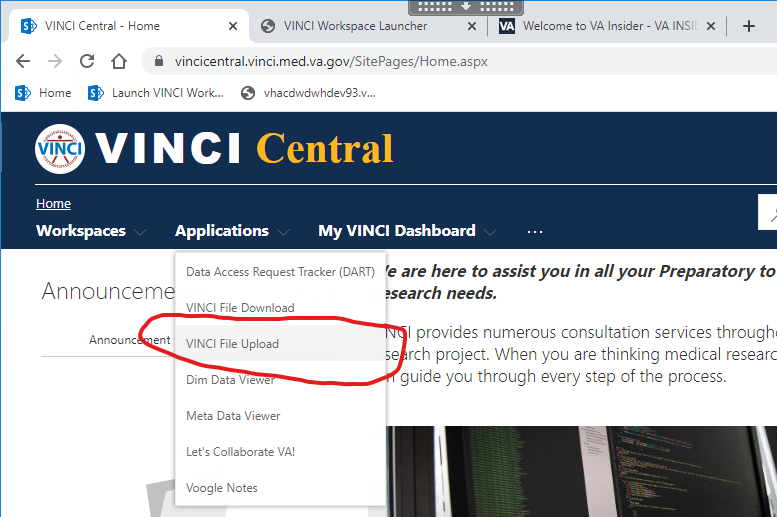
\includegraphics[width=\linewidth]{screenshots/vinci-upload.png}


\section{Download}
If you are unsure, \textbf{DO NOT DOWNLOAD}. The general rule of thumb is any patient related data cannot leave the VINCI servers. So basically only code files clean of PHI, and maybe some plots.



\section{Anaconda\textbackslash Miniconda}
For anaconda and miniconda, the installers are located:

\texttt{P:\textbackslash ORD\_Singh\_2019...\textbackslash Upload\textbackslash Anaconda3-2019.10-Windows-x86\_64.exe}

\texttt{P:\textbackslash ORD\_Singh\_2019...\textbackslash Upload\textbackslash Miniconda3-latest-Windows-x86\_64.zip}


\section{Conda Environments}
Currently we have 3 conda environments set up. To install,\begin{enumerate}
    \item Run \texttt{`conda env list'}
    \item The base environment should be under something of the form \texttt{`\dots\textbackslash envs\textbackslash base'}
    \item Unzip the desired environment to the same \texttt{`\dots\textbackslash envs'} folder. 
    \item After installation, would recommend running \texttt{`python -m ipykernel install --user'} 
\end{enumerate}


\subsection{ahrq}
\textbf{Zip Location: }\texttt{P:\textbackslash ORD\_Singh\_2019...\textbackslash Upload\textbackslash ahrq-probably-pytorch-2021-11.zip}

The most standard conda environment. This environment mainly contains standard anaconda packages such as: numpy, pandas, sklearn, matplotlib, etc. 

It also has \textbf{Torch}. \textbf{NOT PyTorch!!!} Google the difference. 

This environment also can install UMAP and SpaCy by the following:

\subsubsection{UMAP}
In the Upload folder, there is a zip called \texttt{`packagestoinstall.zip'}. Note that this is only useful for the \texttt{ahrq} environment.

\subsubsection{SpaCy \& MedSpaCy}
Did everything with pypi/pip, since MedspaCy is only on pypi. The files needed for installation is all in the upload folder, under the folders ``Upload/spacy'' and ``Upload/medspacy''. Run \texttt{`pip install xxx.whl/xxx.tar.gz'} for all the following packages (in order).

For spaCy:

spacy\_legacy$\rightarrow$ blis$\rightarrow$catalogue$\rightarrow$cymem$\rightarrow$langcodes$\rightarrow$murmurhash$\rightarrow$preshed$\rightarrow$pydantic

$\rightarrow$srsly$\rightarrow$typer$\rightarrow$wasabi$\rightarrow$thinc$\rightarrow$spacy\_loggers$\rightarrow$smart\_open$\rightarrow$pathy$\rightarrow$spacy

For MedspaCy:

spacy$\rightarrow$cython$\rightarrow$quicksectx$\rightarrow$pyfastner$\rightarrow$pyrush$\rightarrow$pysbd$\rightarrow$requests
(Need to downgrade anaconda's default requests package from 2.25 $\rightarrow$ 2.13 due to version conflict\dots)

After the installation I have been getting issues with my Jupiter notebooks. It has been giving me ``Warning: Deprecation Warning, `should\_run\_async' will not call `transform\_cell' automatically in the future \dots'' This most likely is related to the downgrading of requests, but I'm not sure. Also not sure if this broke anything else.

\subsection{ahrq-tf}
\textbf{Prioritize installing the ahrq-tf-bert environment instead now. All packages in that environment are newer}.

\textbf{Zip Location: }\texttt{P:\textbackslash ORD\_Singh\_2019...\textbackslash Upload\textbackslash ahrq-tf-2022-07.zip}

This is a much bigger and much powerful environment than the base ahrq environment. Install based on need.

It contains the following packages and their dependencies:
\begin{enumerate}
    \item Python 3.7
    \item The standard anaconda packages, pandas, sklearn, numpy, etc
    \item TensorFlow 2.1.0.
    \item UMAP
    \item PyTorch
\end{enumerate}


\subsection{ahrq-tf-bert}
\textbf{Zip Location: }\texttt{P:\textbackslash ORD\_Singh\_2019...\textbackslash Upload\textbackslash ahrq-tf-bert.zip}

This environment was created to run Transformers. It was made as an entirely new environment, since \texttt{ahrq-tf} had unresolvable dependency conflicts with Transformers.

It contains the following packages and their dependencies:
\begin{enumerate}
    \item Python 3.8
    \item The standard anaconda packages, pandas, sklearn, numpy, etc
    \item TensorFlow 2.3.0. (With pydot to plot models)
    \item UMAP
    \item PyTorch
    \item Transformers
    \item SpaCy
\end{enumerate}


\section{Creating new Conda environments}
\textbf{A Windows machine/VM is almost a must} for creating new conda environments.
\begin{enumerate}
    \item On the Windows computer, create the conda environment through conda installs. (Using pip install might mess things up)
    \item Run \texttt{`conda pack --format zip'}
    \item Send created zip to Baylor personnel (Andy). 
    \item Baylor personnel uploads to Baylor OneDrive
    \item Baylor personnel download zip onto General Desktop.
    \item Upload zip into dev workspace.
\end{enumerate}

\textbf{REMINDER:} remember to do some basic verification that the packages work as intended. At least try \texttt{`import xxx'}, which fails surprisingly quite often.

\subsection{Big File}
\textbf{If environment zip exceeds 2gb}, the Baylor person needs to do additionally:
\begin{enumerate}
    \item I (Andy) split them on my side using \texttt{`split -b 1900m ahrq-tf-bert.zip'} 
    \item Then I get them to my VA laptop using BCM OneDrive. Then upload to VINCI.
    \item On the VINCI side, I think you can do \texttt{`cat xaa xab > ahrq-tf-bert.zip'}. The order of the 2 arguments matters. Not sure if this is the fastest way to re-join. Might have to use "git bash" or something to get access to cat command (I think this is what I did last time even though it's slow). Might want to validate somehow before unzipping.
\end{enumerate}


\section{Adding Packages to existing Environments}
It is highly recommended to maintain a parallel/mirror environment on an outside desktop with internet access. This way, by running conda install on the outside environment, conda will display a list of missing dependencies that it will install. 

The most important part is getting the dependencies and all the versions correct. 

Once you know all the packages you need, download them on the General Desktop on most likely conda-forge. \textbf{Remember to verify that the name is the exact same}, such as under \url{https://anaconda.org/conda-forge/umap-learn/files}, there are many many similar builds.

After the packages are downloaded on the General Desktop, upload onto Dev and install using \texttt{``conda install xxx.tar.bz2''}.
\end{document}
